
%%=============================================================================
%% H6 - ZPools & VDEV's
%%=============================================================================

\chapter{Zpools \& VDEV's}
\label{ch:h6}

In dit hoofdstuk worden zpools en diens bouwstenen, VDEV's, wat meer toegelicht. Er wordt ook een demonstratie gegeven over hoe men zpools en VDEV's aanmaakt en wijzigt.

\section{VDEV's: Virtual Devices}

\subsection{Concept}

VDEV's (of voluit Virtual Devices) zijn de bouwstenen van storage pools; het zijn een soort van device drivers die elk een bepaalde functionaliteit aanbieden. Er bestaan verschillende soorten VDEV's: zo zijn er bijvoorbeeld striping VDEV's en mirror VDEV's. Ook worden de verschillende RAID-Z-vormen geïmplementeerd met behulp van één of meerdere VDEV's \autocite{ZFSBonwick}.

Conceptueel worden virtual devices voorgesteld in een boomstructuur, waarvan de bladeren de fysieke VDEV's voorstellen; deze VDEV's komen overeen met fysieke apparaten zoals harde schijven. De andere knopen in de boom worden logische VDEV's genoemd omdat ze een groepering vormen van fysieke VDEV's. Zoals in elke boom bestaat er ook in deze structuur van virtual devices een wortel of \textit{root}. De kinderen van deze root VDEV worden de top-level VDEV's genoemd \autocite{Microsystems2006}.

\begin{figure}
  \centering
  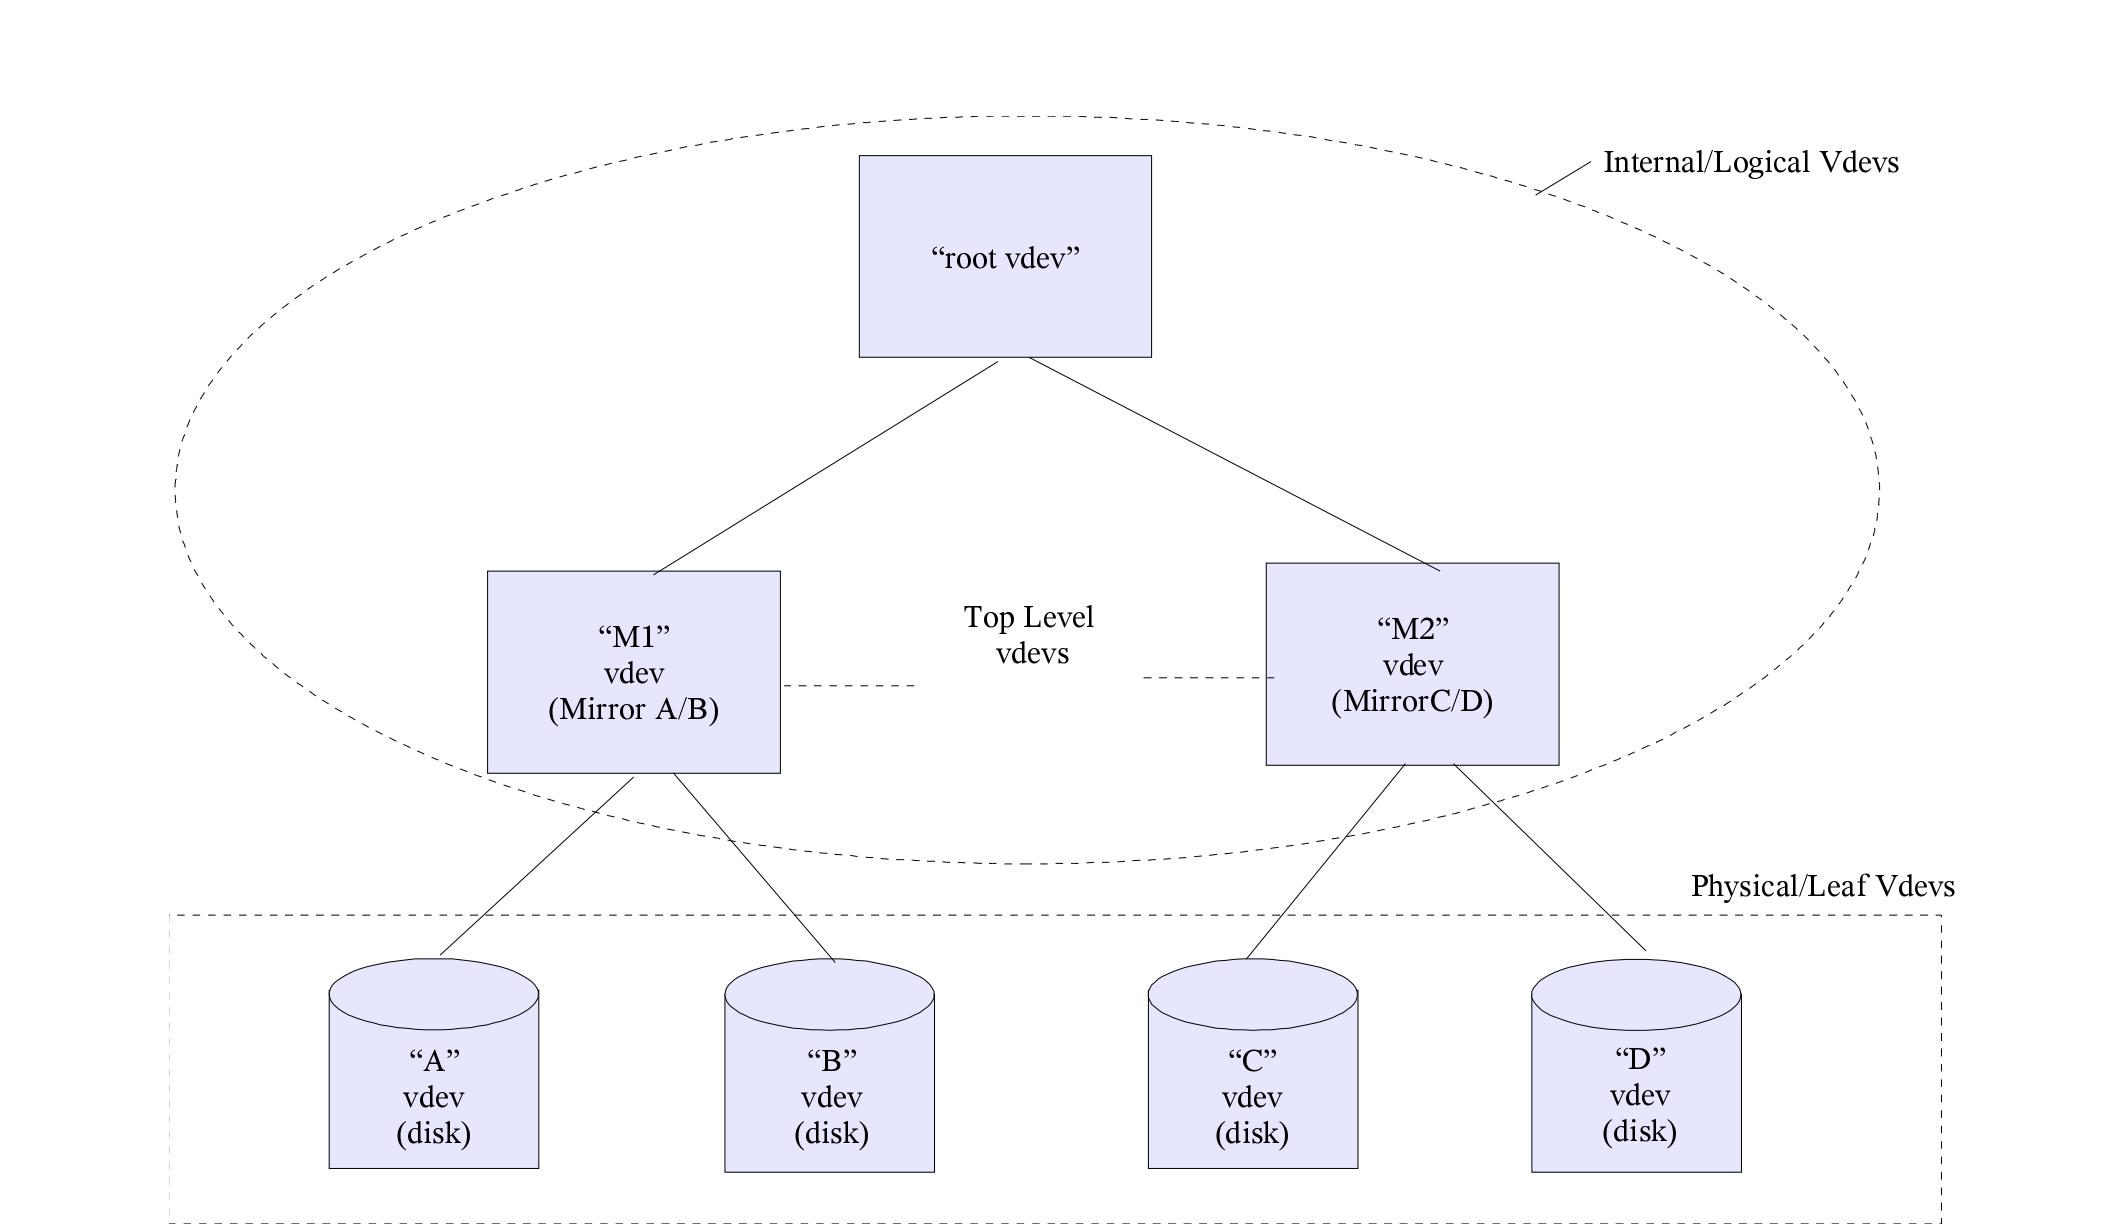
\includegraphics[width=0.9\textwidth]{h6_vdevs_tree}
  \caption{Conceptuele voorstelling van VDEV's in een boomstructuur: M1 en M2 zijn mirrors VDEV's; apparaten A t.e.m. D zijn kinderen van deze VDEV's \autocite{Microsystems2006}.}
  \label{fig:vdevs_boom}
\end{figure}

\subsection{Speciale VDEV's}

Naast VDEV's voor redundantie en striping bestaan er ook nog andere virtual devices die een specifieke rol vervullen. Deze VDEV's worden ingezet met als hoofddoel de performantie van ZFS naar omhoog te trekken \autocite{Lucas2015}.

\subsubsection{SLOG: Seperate Intent Log}

\section{Storage pools of zpools}

Zoals reeds gezegd in Hoofdstuk \ref{ch:h3} vormen storage pools (of zpools in ZFS-termen) de eerste vorm van abstractie binnen de gehele ZFS-stack: zpools bieden namelijk een interface aan tot de onderliggende fysieke schijven. Het zijn echter VDEV's die ervoor zorgen dat data kan weggeschreven worden van en naar de schijven. Ter verduidelijking kan er een analogie worden gemaakt met een traditionele RAID-controller en de schijven in een RAID-array: zpools vervullen de rol van RAID-controller, terwijl VDEV's de schijven van de 'array' voorstellen. De zpool ('RAID-controller') verdeelt of stripet data over één of meerdere VDEV's ('schijven') \autocite{Lucas2015}.

\subsection{Aanmaken en beheren van zpools}

Het testsysteem waarover we beschikken bevat drie interne harde schijven, elk direct aangesloten op het moederbord met een SATA-kabel. Dit aantal is voldoende om een RAID-Z1 opstelling mee te maken. Vooraleer er echter VDEV's kunnen worden toegevoegd of gewijzigd, moet er eerst een ZFS storage pool worden aangemaakt; er kunnen meerdere storage pools worden aangemaakt, maar in ons geval is één storage pool meer dan voldoende.

\subsubsection{Bekijken van aanwezige pools}

Voor het beheer van pools wordt er gebruik gemaakt van het commando \texttt{zpool}. Om bijvoorbeeld de huidige zpools te bekijken, geeft men het volgende commando in:

\begin{lstlisting}[language=bash,style=command_style]
$ zpool list
no pools available
\end{lstlisting}

\subsubsection{Aanmaken van een nieuwe pool}

Op dit moment zijn er nog geen pools aangemaakt, dus de uitvoer van bovenstaand commando is normaal. Om een zpool aan te maken met de drie schijven waarover we beschikken, gebruik je het volgende commando:

\begin{lstlisting}[language=bash,style=command_style]
$ zpool create storage /dev/sda /dev/sdb /dev/sdc
\end{lstlisting}

Deze instructie maakt een zpool aan met de naam 'storage'. Vervolgens kan je een lijst opvragen van alle pools die op het systeem aanwezig zijn:

\begin{lstlisting}[language=bash,style=command_style]
$ zpool list
NAME      SIZE  ALLOC   FREE  EXPANDSZ   FRAG    CAP  DEDUP  HEALTH 
storage  2.27T   154K  2.27T         -     0%     0%  1.00x  ONLINE 

(deel van de uitvoer is weggelaten)

\end{lstlisting}

De uitvoer van dit commando geeft reeds enkele eigenschappen van de pool weer, zoals de naam, de totale grootte van de pool, de gebruikte ruimte van de pool, de vrije ruimte en de hoeveelheid fragmentatie. Een andere eigenschap die interessant kan zijn, is DEDUP of deduplicatie: indien er verschillende kopieën zijn van een stuk data, dan houdt ZFS deze maar één keer bij. 

\subsubsection{Gezondheid van pools}

Om de gezondheid en structuur van een pool na te kijken, gebruik je het commando \texttt{zpool status}:

\begin{lstlisting}[language=bash,style=command_style]
$ zpool status
  pool: storage
 state: ONLINE
  scan: none requested
config:

	NAME        STATE     READ WRITE CKSUM
	storage     ONLINE       0     0     0
	  sda       ONLINE       0     0     0
	  sdb       ONLINE       0     0     0
	  sdc       ONLINE       0     0     0

errors: No known data errors
\end{lstlisting}

Dit commando geeft een overzicht van de interne structuur en gezondheid van elke pool op het systeem, samen met de aanwezige VDEV's. Het merendeel van de uitvoer spreekt voor zich: 'pool' geeft de naam van de pool weer en 'state' geeft de algemene toestand van een pool weer. De eigenschap 'scan' geeft aan of er een zogenaamde scrub wordt uitgevoerd of uitgevoerd is geweest. Een scrub is een scan die kan worden uitgevoerd door ZFS om de consistentie en integriteit van de pool na te gaan; indien mogelijk worden fouten automatisch gerepareerd. Een scrub is dus in principe de equivalent voor een \texttt{fsck} binnen ZFS. De vijf kolommen onder de eigenschap 'config' geven informatie over de VDEV's van de pool weer; de drie kolommen aan de rechterzijde geven het aantal fouten aan dat door een bepaald VDEV werd gedetecteerd.

\subsubsection{Eigenschappen van pools}

Zoals reeds gezegd in Hoofdstuk \ref{ch:h3} is ZFS grotendeels een objectgeoriënteerd bestandssysteem. Elk object binnen ZFS heeft bepaalde eigenschappen (properties); deze kunnen dan ook worden opgehaald en gewijzigd. Het is dan ook niet verwonderlijk dat zpools tevens objecten zijn, met elk bepaalde eigenschappen.

Om bijvoorbeeld alle eigenschappen van een pool op te halen, gebruikt men het commando \texttt{zpool get all <naam van de pool>}:

\begin{lstlisting}[language=bash,style=command_style]
$ zpool get all storage
NAME     PROPERTY                    VALUE                       SOURCE
storage  size                        2.27T                       -
storage  capacity                    0%                          -
storage  altroot                     -                           default
storage  health                      ONLINE                      -
storage  guid                        2498162094782357460         default
storage  version                     -                           default
storage  bootfs                      -                           default
storage  delegation                  on                          default
storage  autoreplace                 off                         default
storage  cachefile                   -                           default
storage  failmode                    wait                        default
storage  listsnapshots               off                         default

(deel van de uitvoer is weggelaten)
\end{lstlisting}

Indien men een eigenschap van een pool wilt wijzigen, gebruikt men het commando \texttt{zpool set <eigenschap>=<waarde> <naam van de pool>}: 

\begin{lstlisting}[language=bash,style=command_style]
$ zpool set comment="Testpool" storage
$ zpool get comment storage
NAME     PROPERTY  VALUE     SOURCE
storage  comment   Testpool  local
\end{lstlisting}

In bovenstaand voorbeeld werd de property 'comment' aangepast; vervolgens werd de nieuwe waarde opgehaald.

\subsubsection{Verwijderen van een pool}

Om een zpool en diens VDEV's te verwijderen, gebruik je het commando \texttt{zpool destroy <naam van de pool>}:

\begin{lstlisting}[language=bash,style=command_style]
$ zpool destroy storage
$ zpool list
no pools available
\end{lstlisting}



\subsection{Aanmaken en wijzigen van VDEV's}

In het begin van dit hoofdstuk werd er reeds kort gesproken over VDEV's en hun rol bij zpools: alle redundantie bij RAID-Z zit in feite in deze VDEV's. Het zijn de virtual devices (en dus niet de storage pools) die het maken van een RAID-opstelling binnen ZFS mogelijk maken \autocite{Lucas2015}.


